% !Mode:: "TeX:UTF-8"

\documentclass[12pt]{apmcmthesis}

\usepackage{url}
\usepackage{ctex}
\usepackage{graphicx}
\graphicspath{{},{figures/}}

%%%%%%%%%%%%填写相关信息%%%%%%%%%%%%%%%%%%%%%%%%%%
\tihao{A}                            %选题
\baominghao{2201046}                 %参赛编号
\begin{document}
\bibliographystyle{plain}
\pagestyle{frontmatterstyle}

\begin{abstract}
	
In order to extract characteristic information such as temperature and crystallization progress in an image, this paper built two models.\textbf{Model one}:
Image Sequence generation based on\textbf{ Pix2pix of GAN }model. The model is able to generate an image of the next second based on the image of the previous second.\textbf{ Model Two:}Melting Crystallization prediction model based on \textbf{Resnet18}.The model can predict the temperatures of No.1 thermocouple and predict the progress of crystallization\textbf{ (0-100\%)}.

For problem 1: \textbf{The first step} is to crop the $101\times 55$ pixel position in the upper left corner of the image; \textbf{In the second step},\textbf{ Baidu Paddlepaddle open source framework PaddleOCR} is used to identify the text in the cropped picture, then processed data  of the recognized text, and the temperatures of No.1 thermocouple and No.2 thermocouple are extracted and automatically saved to Annex 2.

For problem 2:\textbf{ Model One:}Calculate the average of each photo and plot the time series. It find that the average value reaches the maximum value when it form completely melting state to the molten state, as well the average value drops sharply when it from  the molten state to  crystallization state, corresponding to the maximum value in the first-order difference of the picture of average time series. \textbf{Model Two:}Selecting the point of \textbf{$(803,661)$} in each picture , then establishing the time series model  using the values of the three channels and the sum, and it is found that the red channel value begins to reach the maximum, and the blue channel value  begins to reach the minimum reaction when it is complete melting; The green channel value reaches its maximum than it reaches a fully molten state and begins crystallizen.

For question 3: Through question 2, It is found that the picture contains  information of the temperature of the reaction and the crystallization progress. \textbf{Therefore}, consider using CV to establish the functional relationship between the  temperature and time. \textbf{Firstly}, \textbf{the Pix2pix based on GAN } is used to establish the relationship between image and time,  the model can use the image  of the previous image to predict and generate  the next image;
A functional relationship between the image to the temperatures of No.1 thermocouple and the crystallization progress is established by Using a neural network based on \textbf{Resnet18},. Through the above two models, the implicit function relationship of \textbf{time-image-temperature-crystallization} progress is established as a whole.


\keywords{GAN\quad  Pix2pix\quad   Resnet18\quad  Neural networks \quad  PaddleOCR}
\end{abstract}



\newpage
%目录
\tableofcontents


\newpage
\pagestyle{mainmatterstyle}
\setcounter{page}{1}
\section{Introduction}
\subsection{Problem Background}
The continuous casting process is a production process in the foundry industry in which a mold flux is added to the molten steel surface in the crystallization agent. The metallurgical function of the crystallization agent is mainly determined by its melting rate and crystallization rate under the temperature control curve. Only when the molten liquid residue has a good glass state can the lubrication function of the slag film be guaranteed. If the crystallization temperature of the liquid slag is high, it is easy to precipitate crystals, which is not only detrimental to solid friction, but also cannot increase the shear force in the liquid slag film. Therefore, it is very important to observe the phase in the crystallization process to judge the quality of the crystallization agent, a good crystallization agent can not only improve product quality, but also reduce production costs.

However, because 1 image is produced every 1 second during the experiment, each set of experiments will produce about 700 adjacent images, which greatly increases the workload of the experimenter, and because the experimenter only focuses on 6 nodes, a lot of valid information has not been unearthed, and the privacy protection of the independent intellectual property rights of the device itself, resulting in incomplete data capture, the need to rely on manual screening and identification records after the end of the test, wasting a lot of manpower

Therefore, it is necessary to establish a model to solve the problem of data identification and recording, extract image features, facilitate staff to better understand the melting and crystallization process, conduct follow-up analysis, and reduce the workload of experimenters.
\subsection{Problem analysis}
Question one  Due to the fixed size of each photo, the size and position of the text part in the upper left corner are fixed, but the text information that needs to be intercepted accounts for too small a proportion of the given picture, which is easy to produce errors during text recognition, reduce the accuracy, in order to reduce the complexity of the algorithm and improve the computer computing power, the picture needs to be preprocessed, the image segmentation algorithm is used to crop out the sub-image containing text in the upper left corner of the original picture, and then use the PP-OCRv3 model to identify the text in the sub-image. After extracting the text, the extracted text is processed and the corresponding and correct data is saved in Annex 2. Based on Annex II of the data already filled, a temperature-time curve can be created to determine which thermocouple has an inaccurate test result.

Question two  In order to explore the dynamic difference of adjacent sequence images in the process of crystallization and melting, it is necessary to model adjacent images and perform time series analysis, and the difference correlation coefficient of adjacent images can be considered for modeling. And consider using the pixels of a certain point to study the change relationship or the average and variance of the picture to study the change relationship. Therefore, consider using the average of each photo, building a time series model and selecting a point in each picture, using the value of the three channels of RGB and the sum of the three channels to build a time series model to solve the problem.

Problem three  The picture contains a lot of information, if the second question can get a significant correlation between the mean of the image, pixels and temperature, complete melting point, complete melting, and beginning of crystallization, you can consider using a generative model to generate a picture after a period of time based on the previous photo and the time difference. Assuming that the melting rate and crystallization rate are equal, that is, the average rate is used instead of the instantaneous rate, then by labeling the stage in which the picture is located, the reaction accounts for the percentage of reaction completion, and the functional relationship between the picture and the temperature, the stage, and the reaction progress can be established by training the neural network.

\subsection{Question restatement}
Problem one  In the first step, segment the upper left corner of the image; The second step is to use the OCR recognition tool to identify the text; In the third step, perform data processing on the recognized text and automatically save the data to a file

Problem two  Select suitable indicators, extract the features and differences between adjacent images, study the dynamic differences between adjacent sequence images during the melting and crystallization of liquid residue, and quantify the differences. On this basis, a time series model is established and the image is analyzed to obtain the correlation curve.

Problem three  Establish a generative model, generate a picture after a period of time based on the last picture and the time difference, so as to establish a picture-time functional relationship; assume that the melting rate and crystallization rate are equal, replace the instantaneous rate with the average rate, mark the stage at which the picture is located, the reaction accounts for the percentage of reaction completion, and train the neural network to establish the functional relationship between the picture to temperature, stage, and reaction progress.. Thereby establishing the functional relationship of picture-temperature, picture-stage, picture-reaction progress.

\section{Model building and solution of question one}

\subsection{Data preprocessing}
\setlength{\parindent}{2em} Since the size of each photo is fixed, the size and position of the text part in the upper left corner are fixed, and the proportion of text in the whole picture is too small, In order to avoid the error caused by the small proportion of text
and reduce the complexity of the algorithm, improve the computer computing power, consider cutting out the upper left text part from the original image for further processing. The image matrix is read into the computer, and the sub-image containing text in the upper left corner of the original picture is cropped out by using the image segmentation algorithm, and the sub-image is recognized and cropped out by the 101*55 pixels in the upper left corner of the original image when cropping.
The cropped subimage is shown in Figure 1:

\begin{figure}[htbp]
	\centering
	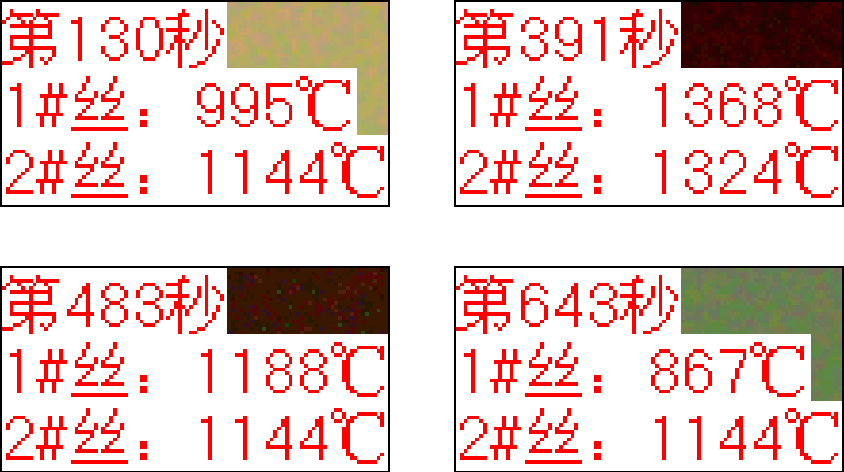
\includegraphics[scale=0.3,angle=0]{1.png}
	\caption{Cropped picture}
	\label{a}
\end{figure}


\subsection{Text recognition}
\setlength{\parindent}{2em} Question 1 requires that the time and temperature data in the upper left corner of each image be automatically extracted and automatically imported into the corresponding table in Annex 2. In order to meet this requirement, we use the PP-OCRv3 model in the paddleOcr framework of PaddlePaddle open-source framework to identify the text in the cropped picture, extract the text and process the extracted text, and save the corresponding and correct data to Annex 2.
\subsubsection{PaddlePaddle open source framework PaddleOCR introduced}
\setlength{\parindent}{2em}PaddleOCR \cite{1}is the industry's smallest ultra-lightweight 8.6M Chinese and English recognition OCR model suite open source by PaddlePaddle , which has been streamlined and optimized on the basis of re-realizing academic algorithms and taking into account the balance between accuracy and speed.

\setlength{\parindent}{2em}PaddleOCR supports a variety of cutting-edge algorithms related to OCR, including rich text detection, text recognition and end-to-end algorithms, and develops industry-featured models/solutions PP-OCR and PP-Structure on this basis, opening up the whole process of data production, model training, compression, inference and deployment.
\subsubsection{Introduction of PP-OCR}
\setlength{\parindent}{2em}PP-OCR is a series of models proposed by PaddleOCR combined with real scenarios and industry experience, selecting DB \cite{2}and CRNN \cite{3} as the basic detection and identification model, and after a series of optimization strategies, a series of models are proposed, which are often used in industrial applications .And the PP-OCR model forms a model library in different languages for general scenarios

\begin{figure}[htbp]
	\centering
	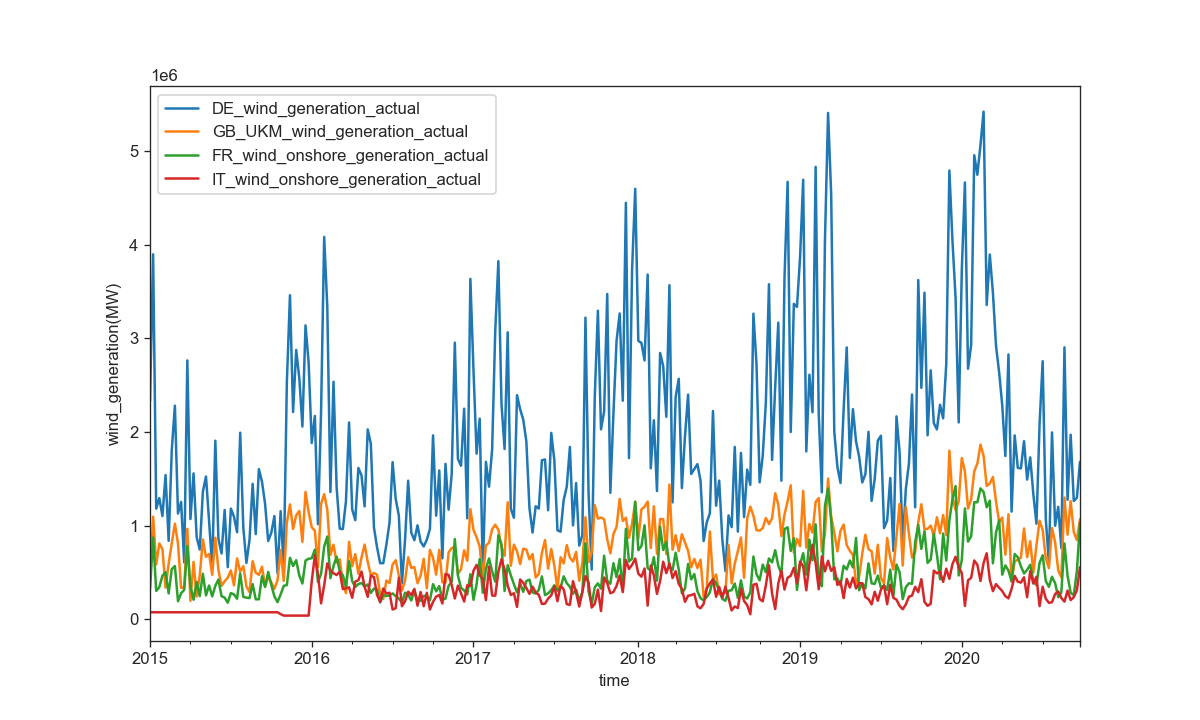
\includegraphics[scale=0.7,angle=0]{2.png}
	\caption{PP-OCR process}
	\label{a}
\end{figure}

\setlength{\parindent}{2em}Compared with previous PP-OCR models, the PP-OCRv3 model greatly improves the accuracy of various scenarios when the speed is comparable.

\setlength{\parindent}{2em}Among them, the operation process of PP-OCRv3 model is to detect the text in the picture after entering the picture, extract the detected text and recognize it, and finally convert the recognized text into text output, the model includes text detection and text recognition. Figure 2 shows the text detection and recognition process.

\setlength{\parindent}{2em}The PP-OCRv3 detection model is an upgrade of the CML collaborative learning text detection distillation strategy in PP-OCRv2. The core idea of CML combines (1) the traditional Teacher instructs Student's standard distillation and (2) the DML mutual learning between the Students network, which allows the Student network to learn from each other while the Teacher network guides. PP-OCRv3 is further optimized for teacher model and student model, respectively. Among them, when optimizing the teacher model, the PAN\cite{5} structure LK-PAN of the Big Receptive Field is proposed and the DML distillation strategy is introduced. In the optimization of the student model, the FPN\cite{6} structure RSE-FPN of the residual attention mechanism is proposed. Compared with the previous PP-OCR model, the detection accuracy has been greatly improved.

\setlength{\parindent}{2em}The recognition module of PP-OCRv3 is optimized based on the text recognition algorithm SVTR. The recognition module no longer adopts CRNN, but is replaced by the newly included text recognition algorithm SVTR \cite{7} in IJCAI 2022, which by introducing the Transformers structure, the context information of the text line image is more effectively mined, so as to improve the text recognition ability.

\setlength{\parindent}{2em}Among them, SVTR is a new text recognition model proposed this year that can complete the text recognition task by relying only on visual features, which has the advantages of high precision and fast speed. And in Chinese scenario, the recognition task performed excellently, reaching SOTA. It solves the problem of poor performance caused by the complex design of the previous text recognition model (extracting visual features), sequence model (for transcription), and language model.


\subsubsection{Use the framework to identify the results}
\setlength{\parindent}{2em}As shown in the figure, the effect of using paddleocr recognition, the left side is the text recognition result, each picture paddleocr can detect three targets and draw a border, and the right side is the text recognition result, including the confidence of recognition.
\begin{figure}[htbp]
	\centering
	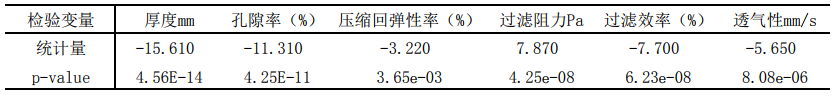
\includegraphics[scale=0.3,angle=0]{3.png}
	\caption{Identify the results}
	\label{a}
\end{figure}

\subsection{Overall process}
On the basis of the previous step, the recognized text is processed for data processing, and the correct data is automatically saved to Annex 2. The operation documentation of the whole process is as follows:


\textbf{Input}:The picture given by the question. 

\textbf{Output}:The time in the top left corner of the picture、Temperature of number one thermocouple and Temperature of number two thermocouple. 

1.Import the pictures, use the os.listdir function to get the name of all the images in the folder and connect to the folder path to read all the images. 

2.Cut the upper left text information section corp(1, 1, 102, 56) and save with the original file name. 

3.Call Baidu PaddlePaddle text recognition API, ocr=PaddleOCR, PaddleOCR model for text recognition. The model inputs a picture, recognises and returns text information in the picture. 

4.Batch read the text message images saved in Step 2. 

5.The text information images were inputted into the PaddleOCR model one by one, and three strings were identified. 

result=ocr.ocr(image)

data1=int(result[0][0][1][0][1:-1])

data2=result[0][1][1][0][3:9]

data3=result[0][2][1][0][3:9]

6.The text information is extracted by judgment. The first string intercepts the three digits of [1:4] directly as time, no further judgment is required, the second and third strings, starting with the character 'si',  are judged character by character backwards,

if the character is not a number, delete it, at the same time from the back to the front character one by one, delete the end of the string of non-numeric characters. 
while True: [data2=data2[1:] if data2 the first character is not a number], [data2=data2[:-1] if data2 the last character is not a number],
[data3=data3[1:] if data3 the first character is not a number], [data3=data3[:-1] if data3 the last character is not a number]

7.Store the identified information into the dataframe. 

8.The dataframe is stored in Attachment 2, indexed by the identified time, corresponding to the time in Attachment 2.


The first 10 lines of the final recognition result are shown in the following figure:

\begin{center}
\begin{tabular}{lrrrr}
	\toprule
	{} &  NO &  Time &  1\# Temperature &  2\# Temperature \\
	\midrule
	0 &   1 &   110 &             900 &            1142 \\
	1 &   2 &   111 &             904 &            1146 \\
	2 &   3 &   112 &             910 &            1146 \\
	3 &   4 &   113 &             914 &            1144 \\
	4 &   5 &   114 &             918 &            1144 \\
	\bottomrule
\end{tabular}
\end{center}


\subsection{Curve of temperature vs. time}
Temperature-time curve made according to the identified results (1\# wire temperature-2\# wire temperature-time curveLine plot;1\# line average temperature-2\# line average temperature-time graph) As shown in the figure below:This can be seen in Figure 4:
\begin{figure}[htbp]
	\centering
	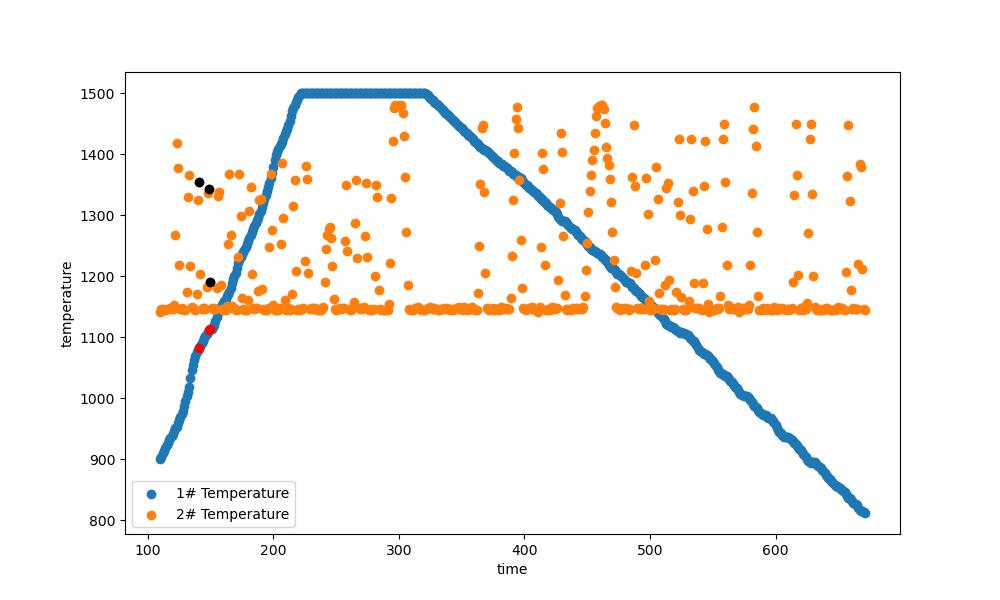
\includegraphics[scale=0.3,angle=0]{4.jpg}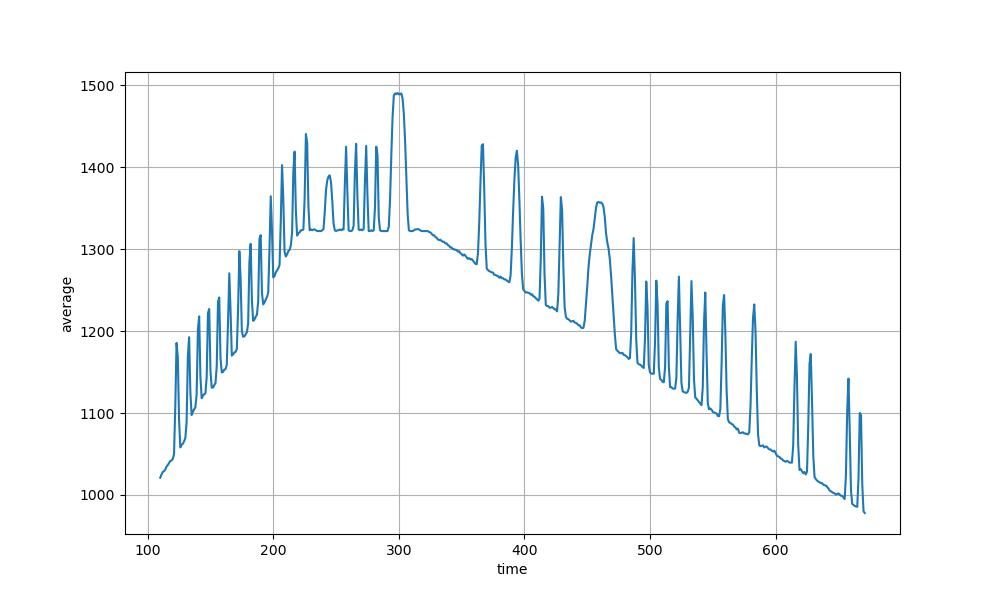
\includegraphics[scale=0.3,angle=0]{5.jpg}
	\caption{1\# wire temperature-2\# wire temperature-time curveLine plot;1\# line average temperature-2\# line average temperature-time graph}
	\label{a}
\end{figure}
The test results of the 2\# silk are inaccurate. Over time, the temperature of the 1\# filament gradually increases, and the curve tends to level off when the temperature reaches 1500, and after a period of time, the curve begins to slowly decline until the end of crystallization. The overall temperature shows a trend of rising-leveling-decreasing, which is consistent with the overall trend of Figure 5 compared to the 1\# filament temperature and average temperature-time plot, so the test results of 1\# silk are accurate. The 2\# silk temperature data is inaccurate, and the 2\# Silk data There are changes in cyclical trends, and the distribution span is large, which can obviously show that the degree of correlation with the average data trend is small. Although most of the points on the curved line are concentrated on a straight line between 1100 and 1200, there are still many data distributed above and below the line in a discrete state (most of them are scattered in the upper part of the line), so the test results of the 2\# filament are inaccurate.
\section{Model building and solution of question two}
In order to quantify the features between adjacent images, the average of the images and the data of a point channel on the image are selected for study. Model 1: Find the average value of each photo, establish a time series model, and draw a graph of the relationship between the mean of the photo pixel points and time for analysis. In the second model, the points (803,661) in each picture are selected, and the time series model is established by using the values of the three channels and the sum of the three channels, and the R-time relationship diagram, G-time relationship diagram, B-time relationship plot and the relationship between the total value of coordinate points and time are drawn for analysis.

\subsection{Image mean model}
The picture can be seen as a superposition of three layers of two-dimensional arrays, each of which is a channel. In a defined RGB color space, each pixel pixel has three layers of value, and these three layers of value represent the value of the point on the three channels, and the computer determines the color of this pixel according to these values.

Assuming that the height of the picture is $ H $ and the width is$  W $, the matrix of the three channels of the image $ (R, G, B) $ is represented as:
$$A  \{A_1,A_2,A_3\} $$Then the average value of the $ i(i=1,2,3,...,562) $ photo is:
$$E(A) = \frac{1}{3 * W * H} \sum_{c=1}^{3} \sum_{i=1}^{H} \sum_{j=1}^{W} A c_{ij}$$
The average value of the image represents the overall brightness of the image. The larger the average value is, the brighter the image will be. So let's figure out take the average of each photo and model the time series. The values of the three channels of the image are extracted, and the values are added and averaged to get the average value of an image.Calculate the mean value of all images and draw the graph of the relationship between the mean value and time. The three red dots successively represent the three points of complete melting, complete fusing and crystallization.Graph of mean versus timeis shown in the figure below:
\begin{figure}[htbp]
	\centering
	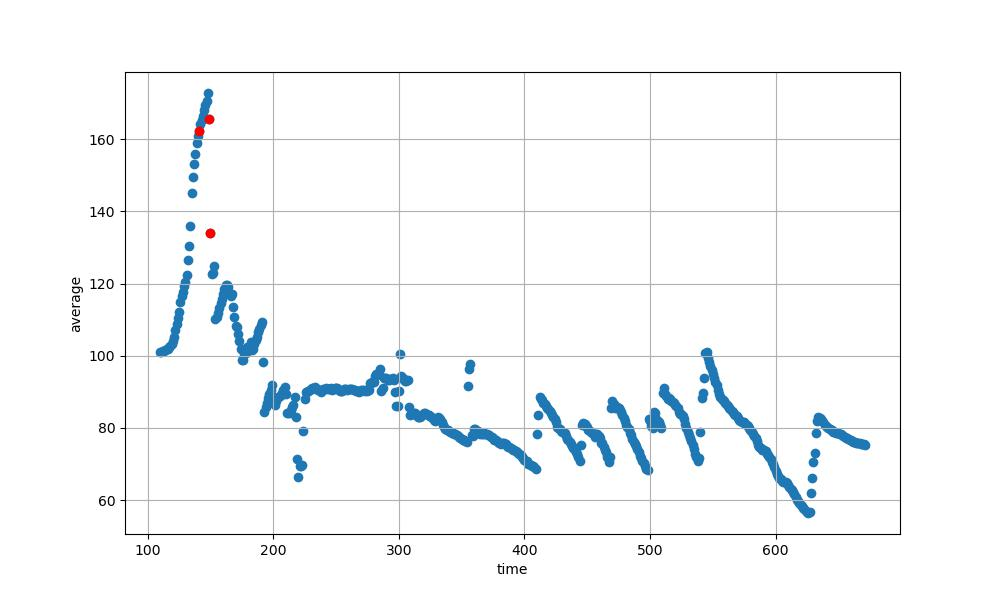
\includegraphics[scale=0.5,angle=0]{6.jpg}	
	\caption{Image mean-time plot}
	\label{a}
\end{figure}

As can be seen from the figure, in the process of crystallization and melting, the average pixel of the image continues to rise after complete melting until it reaches the peak, and then begins to decline to the point of complete melting. It can be seen that the average pixel of the point of complete fusing is higher than that of the point of complete melting, and then the pixel continues to decline to the point of crystallization.
It can be seen that the relationship between the average pixel values of the three points is: complete fusing > complete melting > beginning crystallization.That is, among these three points, the picture that is completely fused has the highest brightness, followed by complete melting, and the brightness that begins to crystallize is the lowest.


\begin{figure}[htbp]
	\centering
	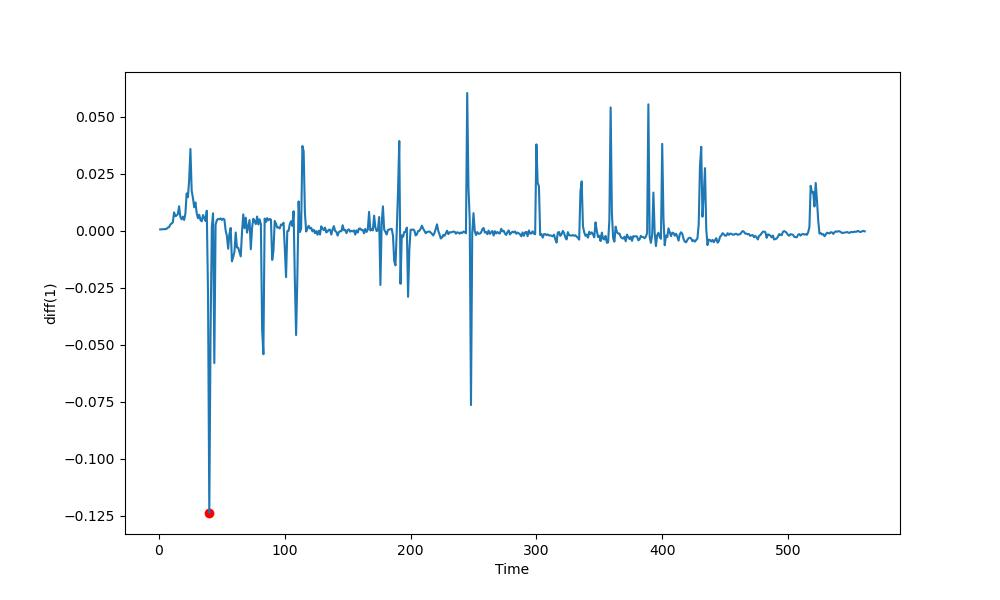
\includegraphics[scale=0.5,angle=0]{7.jpg}
	\caption{First-order differential-time plot of the image mean}
	\label{a}
\end{figure}
Drawing the first-order difference plot of the mean is shown in the figure, combined with Figure 6, it is found that the average value reaches a maximum when it completely melts to the molten state, and the average value drops sharply when crystallization begins from the molten state, which corresponds to the maximum value in the first-order difference of the picture average time series

\subsection{Channel change model}
$ RGB $color mode is a color standard in the industry, which is used to obtain a variety of colors by changing the three color channels of red (R), green (G) and blue (B) and superimposing them on each other. RGB represents the color of the three channels of red, green and blue, and this standard includes almost all the colors that human vision can perceive. It is one of the most widely used color systems.

Suppose the point (H, W) on the image is selected, then its summation formula is
$$sum =  \sum_{c=1}^{3} A c_{hw}$$
Using the RGB tri-color value of a certain point of the image for comparison can also carry out effective analysis of the image.The process is to extract the three values of RGB on the coordinates of each image (803,661) separately, and draw the R-time relationship plot, G-time relationship plot, and B-time relationship plot.Then the three values are summed up to draw the relationship between the total value of coordinate points and time.The three red dots represent the three times at which the melting, the melt, and the crystallization begin.Finally, the information graph on the image coordinate point (803,661) is shown in Figure 8:
\begin{figure}[htbp]
	\centering
	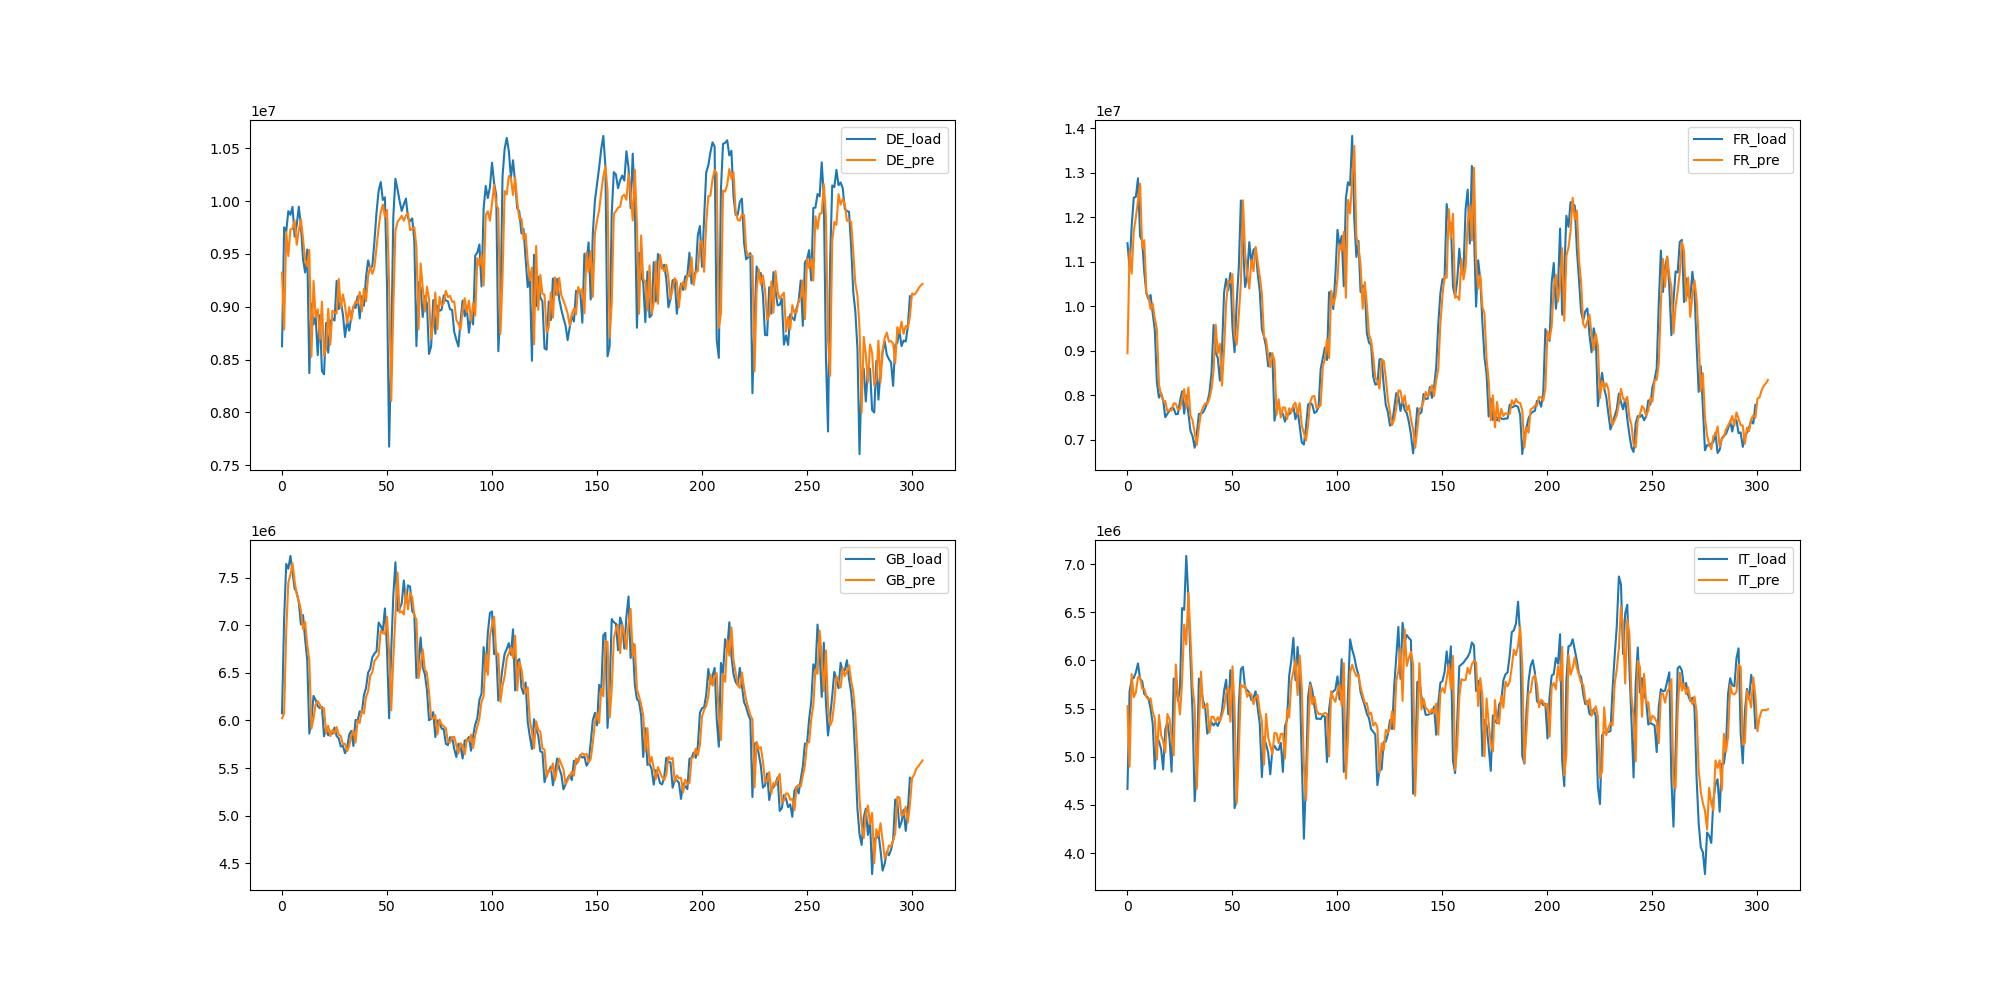
\includegraphics[scale=0.4,angle=0]{8.jpg}
	\caption{Channel-time graph}
	\label{a}
\end{figure}
In the R-time relationship diagram, the curve shows a trend of rapid rise, then stable and finally downward, in which the three points of complete melting, complete fusing, and beginning of crystallization are concentrated in the stable stage after the curve rises to the maximum.

In a G-Time plot, the data  fluctuation distribution. The general trend is to rise rapidly to the peak and then slowly descend, in which the point of complete melting occurs when the curve rises rapidly and reaches the peak, the point of complete fusing appears after reaching the peak, and the point of beginning to crystallize is seen when it begins to fall, where the point of complete melting is almost the same as the point of beginning crystallization, and the point of complete fusing is higher than these two points.

In the B-time plot, the curve tends to go down, then smooth out, and then rise. The three points of complete melting, complete fusing, and beginning of crystallization are concentrated in the stationary stage after the curve drops to the minimum value.

In a total value-time plot, data fluctuations are distributed. The general trend is to rise rapidly to the peak and then slowly decline, and after a period of decline, it begins to decline rapidly. Among them, the point of complete melting appears when the curve rises rapidly and reaches its peak, the point of complete fusing appears after reaching the peak, and the point that begins to crystallize is seen when it begins to fall. The point where the point of complete melting is almost the same as the point where crystallization begins, and the point of complete fusing is higher than these two points.

On the whole, at the beginning of the heating up, the color of the picture is biased towards red, the red channel value quickly climbs to 1, the blue channel value quickly drops to 0, and the green channel value reaches maximum value near the molten point.


\begin{center}
\begin{tabular}{lrrr}
	\toprule
	{} &  1\# Temperature &  2\# Temperature &       chaneel\_sum \\
	\midrule
	1\# Temperature &        1.000000 &        0.027826 &  0.595810 \\
	2\# Temperature &        0.027826 &        1.000000 &  0.085669 \\
	chaneel\_sum            &        0.595810 &        0.085669 &  1.000000 \\
	\bottomrule
\end{tabular}
\end{center}

Find the Pearson correlation coefficient of channel total value and temperature, and find that the channel total value has a correlation of 0.6 with 1\# Temperature. The change in pixels reflects the change in temperature, and the channel total value has only a correlation of 0.03 with 2\# Temperature. Can be considered independent of each other.


\section{Model building and solution of question three}
In order to study the relationship between image, time, temperature, crystallization process, three models are established for research.Model 1: The GAN-based pix2pix image generation model can predict the image of the next second based on the current image, thereby establishing a time-image function relationship.Model 2: Based on the regression model of Resnet18, the model can predict 1\# Temperature based on the image, thereby establishing the image-temperature function relationship.It is worth noting that 2\# Temperatur is not accurate, so 2\# Temperatur is not used as the modeling object.Model 3: Based on the regression model of Resnet18, the model can predict the crystallization progress according to the image, so as to establish the relationship between the image and the crystallization progress.


\subsection{Brief Introduction of neural network}
Neural network is a kind of model produced by imitating animal neurons, which can be used for classification, regression and other problems, and the model has good effect.Neural networks can theoretically fit arbitrary functions, including nonlinear functions, and are one of the most popular mathematical modeling methods today.
In 1959, two biological scientists discovered that frog neurons receive multiple inputs, including inputs from multiple organs of the frog, but only when a single input reaches a threshold, the output will be produced (the frog will respond to a large stimulus).So computer scientists modeled on the principle and structure of biological neurons to propose the concept of perceptrons.The perceptron can be represented as
$$y=o(\sum_{i=0}^{n} w_{i} x_{i}+w_0),$$Among them

$$	o(x)=\left\{\begin{array}{c}
x ,~~~~x>0 \\
0, ~~~~x \leq 0
\end{array}\right.
$$
\begin{figure}[h]
	\centering
	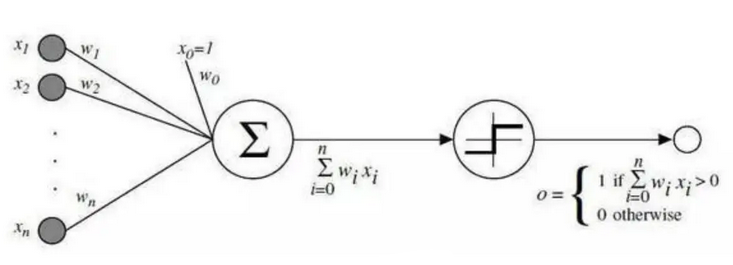
\includegraphics[scale=0.45,angle=0]{93.png}
	\caption{Perceptron}
	\label{93}
\end{figure}
On the basis of perceptrons, scientists set up input layers, hidden layers, output layers, and set up several perceptrons in each layer to form a neural network
\begin{figure}[h]
	\centering
	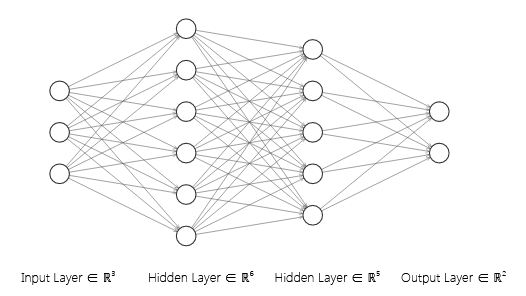
\includegraphics[scale=0.75,angle=0]{94.png}
	\caption{Neural networks}
	\label{94}
\end{figure}
Neural networks use gradient descent to solve optimal values, a class of computer algorithms that solve the minimum values of functions.Assume that hope to solve the objective function 
$ f(x)=f(x_1,\dots ,x_n) $ of the minimum, Assume that hope to solve the objective function  $ x^{(0)}=(x_1^{(0)},\dots ,x_n^{(0)}) $ of the minimum,。 It can start from an initial point  $\alpha > 0$ and build an iterative process based on the learning rate \begin{gather*}
x_1^{i+1}=x_1^{i}+\alpha \frac{\partial f}{\partial x_1}(x^{(i)})\\
\vdots \\
x_1^{i+1}=x_1^{i}+\alpha \frac{\partial f}{\partial x_1}(x^{(i)})
\end{gather*}	 where $x^{(i)}=(x_1^{(i),\dots,x_n^{(n)}}),i>=0$, and the iteration ends once the convergence condition is reached.Figure 10 shows the process of iterating 10 times when solving for the minimum value of \ref{95}$y=x^2$using the shaving descent method, where the dots represent the values after each iteration.
\begin{figure}[h]
	\centering
	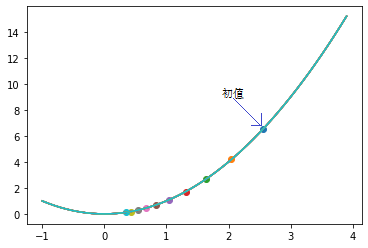
\includegraphics[scale=0.7,angle=0]{95.png}
	\caption{Illustration of the shaving descent method}
	\label{95}
\end{figure}




\subsection{image-to-image:Pix2pix based on GAN}
\subsubsection{Introduction of GAN}
The Generative Adversarial Network\cite{8} is a neural network proposed by Ian Goodfellow in 2014, which is a type of generative network. The idea is that discriminator and optimizer constantly  pitted against each other, and finally make the model reach the Nash equilibrium method. The function to be optimized for adversarial neural networks is:$$\min _{G} \max _{D} V(D, G)=\mathbb{E}_{\boldsymbol{x} \sim p_{\text {data }}(\boldsymbol{x})}[\log D(\boldsymbol{x})]+\mathbb{E}_{\boldsymbol{z} \sim p_{\boldsymbol{z}}(\boldsymbol{z})}[\log (1-D(G(\boldsymbol{z})))]$$where G is the generator and D is the discriminator. GAN is an important model for image style transfer and plays a pivotal role in image generation.

\subsubsection{Introduction to Pix2pix}
Pix2pix\cite{9} is a generative model proposed by Phillip Isola et al. in CVPR2017, which is a kind of adversarial neural network. The author adds a regularization term to the Pix2pix model based on the GAN loss function.The loss function of Pix2pix is:
$$G^{*}=\arg \min _{G} \max _{D} \mathcal{L}_{c G A N}(G, D)+\lambda \mathcal{L}_{L 1}(G)$$Among them$$\mathcal{L}_{L 1}(G)=\mathbb{E}_{x, y, z}\left[\|y-G(x, z)\|_{1}\right],$$
$$ \mathcal{L}_{c G A N}(G, D)=\mathbb{E}_{x, y}[\log D(x, y)]+\mathbb{E}_{x, z}\left[\log (1-D(x, G(x, z))], \arg \min _{G} \max _{D} \mathcal{L}_{c G A N}(G, D)\right. $$Pix2Pix is a style migrator that can complete image conversion in different styles.
\subsubsection{Results of model}
In this paper, the Pix2pix model is used to extract the features between two adjacent pictures, select the adjacent two photos as a set of training data, train 600 epoches, and predict the test pictures.The results are as follows:


\begin{figure}[htbp]
	\centering
	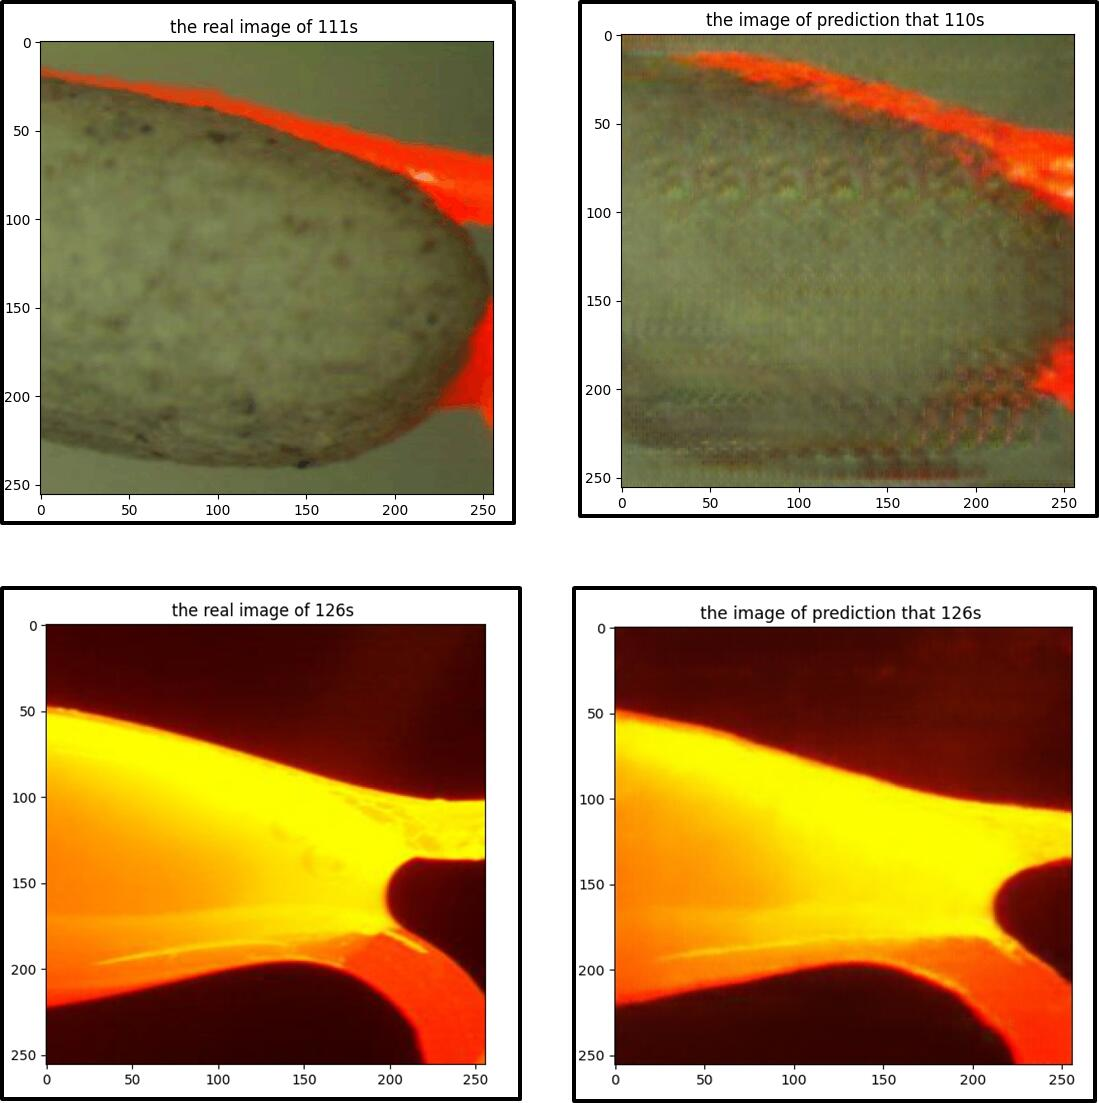
\includegraphics[scale=0.24,angle=0]{9.jpg}
	\caption{Pix2pix prediction picture versus real picture}
	\label{a}
\end{figure}
The figure shows the comparison between the predicted picture and the real picture obtained by using Pixpix to predict the 110 second picture. According to the results, Pixpix can indeed extract the valid information of the current image to generate the next stage of the image.Therefore, Pix2pix is able to extract the feature information of the image and predict the next feature, thus establishing the function relationship between the image and time.
\subsection{image-to-tempreture:Based on Resnet}
Resnet\cite{10} is a neural network based on residual block connection proposed by He Kaiming in 2017, and the basic structure of Resnet residual block is as follows:
$$\mathcal{F}(\mathbf{x}):=\mathcal{H}(\mathbf{x})-\mathbf{x}$$Resnet improves the problem of gradient vanishing and gradient exploding, enabling the network to stack deeper network layers.

Resnet18 is trained using 1\# Temperatur in Annex 2 as the label and the picture as the output. The changing process of the training loss value is as follows:
\begin{figure}[htbp]
	\centering
	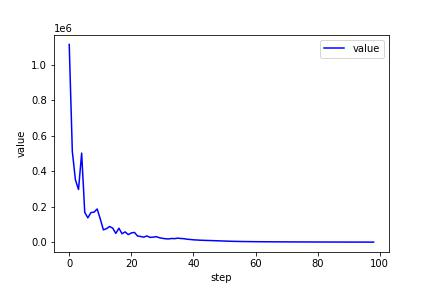
\includegraphics[scale=0.5,angle=0]{10.jpg}
	\caption{train loss}
	\label{a}
\end{figure}

The loss value decreased from 1e6, and although it recovered in the middle, it eventually fell to around 500 and gradually converged, indicating that the model has a good effect.Using the trained model, several of these images are predicted and compared to the real values, and the results are as follows:
\begin{figure}[htbp]
	\centering
	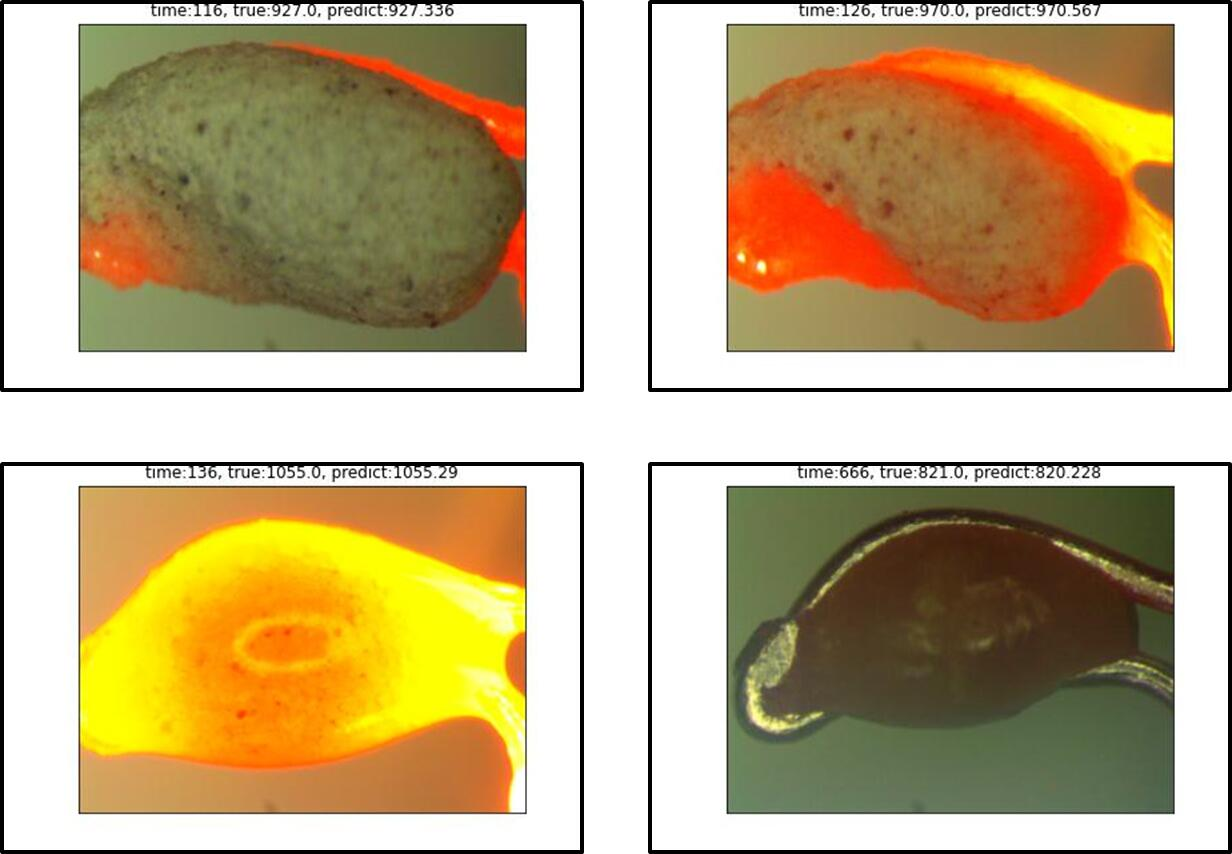
\includegraphics[scale=0.27,angle=0]{11.jpg}
	\caption{true and predict}
	\label{a}
\end{figure}
As can be seen from the figure, the prediction error of the model in each stage of the reaction is small, and the model effect is good.Therefore, Resnet18 can extract the temperature information in the image, thus establishing the image-temperature functional relationship

\subsection{Image-to-crystallization schedule :Based on Resnet}
In order to simplify the process of crystallization reaction, assuming that the crystallization rate is equal during the crystallization process, so the instantaneous crystallization rate can be replaced by the average crystallization rate, and then the progress of crystallization of each picture can be calculated.Assuming that there are N pictures in the crystallization stage, the crystallization progress of the I-th picture is$$C=\frac{i}{N} * 100\%$$.Using the crystallized progress data as labels and all pictures as input, using Resnet to build a regression model, the loss value change process of training is as follows:
\begin{figure}[htbp]
	\centering
	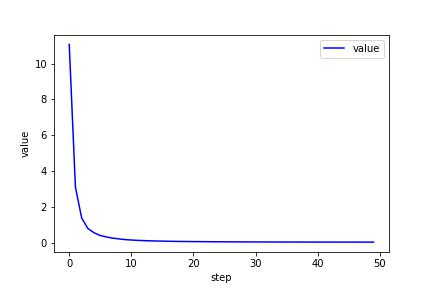
\includegraphics[scale=0.5,angle=0]{12.jpg}
	\caption{true and predict}
	\label{a}
\end{figure}
The loss value of Resnet18 was reduced from 41.9744 to 0.022, and the model achieves convergence effect.Using the trained model to predict several of these images and compare them with the true value, the results are as follows:

\begin{figure}[htbp]
	\centering
	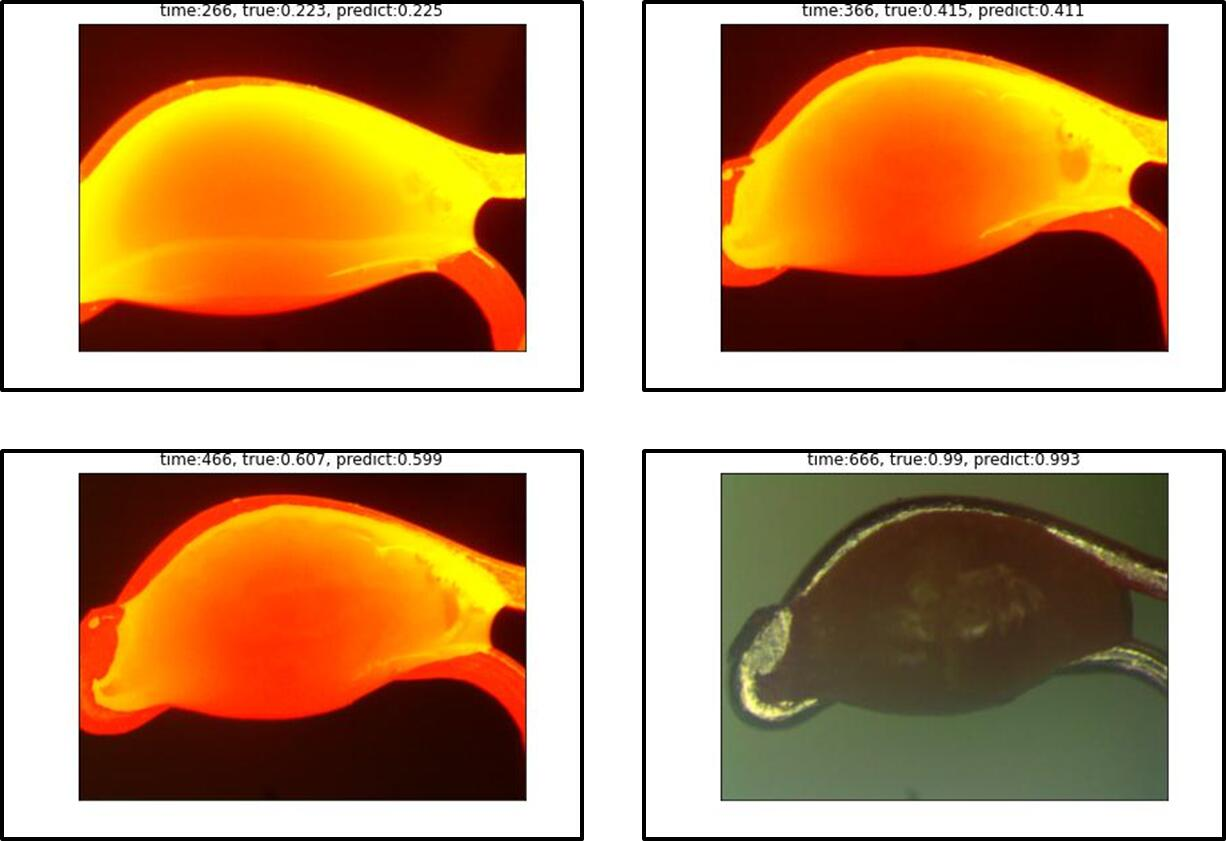
\includegraphics[scale=0.3,angle=0]{13.jpg}
	\caption{true and predict}
	\label{a}
\end{figure}
From the predicted results, it can be seen that the model can extract the crystallization progress information in the image, and has a good effect, so as to establish the image-crystallization progress function relationship.

In summary, this summary uses GAN based Pix2pix model to establish the functional relationship between time and pictures, and uses Resnet18-based neural network to establish the functional relationship between temperature and pictures, crystallization progress and pictures, thus establishing the implicit functional relationship between time, temperature and crystallization on the whole.

\section{Evaluation of the model}
\subsection{The advantages of the model}
\begin{itemize}
	\item Model is simple and practical, can help the staff to reduce the workload
	\item Problem 2 uses a simple model to extract the features of the image
	\item Problem 3 Innovative use of neural networks to study the relationship between attributes
\end{itemize}
\subsection{The disadvantage of the model}

\begin{itemize}
	\item Training the model without a split test set may lead to overfitting
	\item The training time was less, and the effect of Pix2pix did not reach the best
\end{itemize}

\subsection{Model improvement and extension}
\begin{itemize}
	\item Replace the Pixpix model with a better image generation model
	\item Establish the classification model from image to stage
\end{itemize}


%参考文献
\begin{thebibliography}{9}%宽度9
\bibitem{1} \url{https://github.com/PaddlePaddle/PaddleOCR/blob/release/2.5/doc/doc_ch/PP-OCRv3_introduction.md}

\bibitem{2}Minghui Liao, Zhaoyi Wan, Cong Yao, Kai Chen, Xiang Bai.Real-time Scene Text Detection with Differentiable Binarization.CVPR2022.

\bibitem{3}B. Shi, X. Bai and C. Yao, "An End-to-End Trainable Neural Network for Image-Based Sequence Recognition and Its Application to Scene Text Recognition," in IEEE Transactions on Pattern Analysis and Machine Intelligence, vol. 39, no. 11, pp. 2298-2304, 1 Nov. 2017, doi: 10.1109/TPAMI.2016.2646371.

\bibitem{4}S. Bao, Q. Xu, Z. Yang, X. Cao and Q. Huang, "Rethinking Collaborative Metric Learning: Toward an Efficient Alternative without Negative Sampling," in IEEE Transactions on Pattern Analysis and Machine Intelligence, doi: 10.1109/TPAMI.2022.3141095.

\bibitem{5}W. Wang et al., "Efficient and Accurate Arbitrary-Shaped Text Detection With Pixel Aggregation Network," 2019 IEEE/CVF International Conference on Computer Vision (ICCV), 2019, pp. 8439-8448, doi: 10.1109/ICCV.2019.00853.
	
\bibitem{6}T. -Y. Lin, P. Dollár, R. Girshick, K. He, B. Hariharan and S. Belongie, "Feature Pyramid Networks for Object Detection," 2017 IEEE Conference on Computer Vision and Pattern Recognition (CVPR), 2017, pp. 936-944, doi: 10.1109/CVPR.2017.106.

\bibitem{7} Du, Y., Chen, Z., Jia, C., et al.\ 2022, arXiv:2205.00159
	
\bibitem{8} Goodfellow, Ian J., Pouget-Abadie, Jean, Mirza, Mehdi, Xu, Bing, Warde-Farley, David, Ozair, Sherjil, Courville, Aaron C., and Bengio, Yoshua. Generative adversarial nets. NIPS, 2014.

\bibitem{9}P. Isola, J. -Y. Zhu, T. Zhou and A. A. Efros, "Image-to-Image Translation with Conditional Adversarial Networks," 2017 IEEE Conference on Computer Vision and Pattern Recognition (CVPR), 2017, pp. 5967-5976, doi: 10.1109/CVPR.2017.632.

\bibitem{10}K. He, X. Zhang, S. Ren and J. Sun, "Deep Residual Learning for Image Recognition," 2016 IEEE Conference on Computer Vision and Pattern Recognition (CVPR), 2016, pp. 770-778, doi: 10.1109/CVPR.2016.90.
\end{thebibliography}


\newpage

%附录

	\begin{appendices}
	\section{Appendix}
	OCR\_and\_image-to-tempreture.py
	\lstinputlisting[language=python]{code/OCR_and_image-to-tempretrue.py}
	image-to-image-GAN.py
	\lstinputlisting[language=python]{code/image-to-image-GAN.py}
	image-to-Crystallization progress.py
	\lstinputlisting[language=python]{code/image-to-Crystallization progress.py}
\end{appendices}




\end{document} 